%===================================================================================
% Chapter: Introduction
%===================================================================================
\chapter*{Introducción}\label{chapter:introduction}
\addcontentsline{toc}{chapter}{Introducción}
%===================================================================================

\qquad 

La rana \emph{Eleutherodactylus eileenae} (Dunn, 1929) es una especie 
de la familia \emph{Eleutherodactylidae}, endémica de Cuba. 
Se distribuye desde la península de Guanahacabibes, Pinar del Río, 
hasta la Sierra de Najasa, en la provincia de Camagüey. 
Ocupa hábitats como bosques semideciduos, pinares y cafetales
en altitudes de hasta 900 metros sobre el nivel del mar. 
Durante el día permanece oculta en
oquedades de rocas y troncos, y entre la hojarasca y bromelias.
Al caer la noche los machos ascienden 
para vocalizar en ramas y hojas de hasta 3 m de altura. \cite{alonso2001patrones}
En la Figura \ref{fig:colin} se muestra un ejemplar de esta especie, y en la
\href{https://www.fonozoo.com/fnz_detalles_registro_amphibia.php?id=97953&tipo_registro=1}{Guía sonora de los anfibios de Cuba}
se puede encontrar una breve grabación de su canto y otros datos relevantes.\\

\begin{figure}[h!]
    \centering
    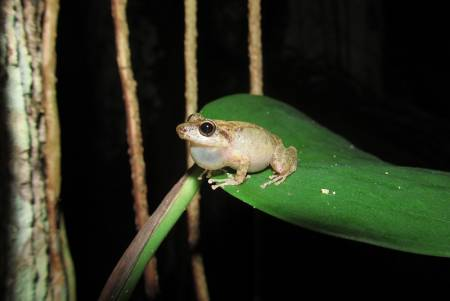
\includegraphics[width=\columnwidth]{Graphics/colin.jpg}
    \caption{Ejemplar de \emph{Eleutherodactylus eileenae}.}
    \label{fig:colin}
\end{figure}


El canto de \emph{E.\,eileenae} consta de dos notas 
diferenciadas: una primera “Co” breve y de frecuencia menor, 
seguida de “Lin” más prolongada y de frecuencia ligeramente 
superior, nombradas de esta forma para imitar el sonido producido. 
Por tal motivo y por simplicidad se procederá a nombrar “Colín” a cada uno de los cantos 
y también se utilizará como nombre coloquial de la especie. 
Estas llamadas median parámetros bioacústicos 
vinculados al estado fisiológico y a la competencia territorial. 
Además, se ha observado que los machos forman agrupaciones 
(“coros”), sincronizando pulsos y modulaciones para incrementar 
la eficacia de atracción de hembras y reducir el riesgo de 
depredación. La presente investigación se centrará en el estudio de dichos
coros y los cantos con fines de apareamiento de los Colines.



\section{Características del \emph{dataset} de grabaciones}

El canto de \emph{E.\,eileenae} se produce en la noche,
cuando los machos se agrupan para vocalizar, 
con picos de actividad en los meses calurosos y lluviosos del año y 
en las horas de la tardenoche y la madrugada.
Con el objetivo de adquirir datos para los estudios de la especie,
el grupo de investigación dirigido por el Dr. Roberto Alonso, de la Facultad de Biología de la Universidad de La Habana,
realizó un conjunto de grabaciones de campo en la zona de la 
Reserva de la Biosfera “Sierra del Rosario”. Después de identificar ciertos
individuos y los sitios donde usualmente se ubicaban para emitir sus cantos, se colocaron
9 micrófonos (cada uno aproximadamente a 1 metro de distancia de su Colín más cercano)
cuya activación remota permitió el registro de la información acústica del coro en cuestión.
Todos los dispositivos eran del mismo modelo, unidireccionales, y eran activados simultáneamente para comenzar a grabar
58 minutos consecutivos, utilizar 2 minutos para guardar los datos adquiridos y luego volver a comenzar a grabar.
Esto se hizo durante 3 noches, en los períodos comprendidos entre las 18:00 horas y las 6:00 horas del día siguiente, entre los días
20 y 23 de octubre de 2023. En la Figura \ref{fig:map} se muestra la distribución geográfica de los micrófonos en el área de estudio.
Como se puede apreciar, los micrófonos fueron colocados en un área con un radio de aproximadamente 20 metros.\\

\begin{figure}[h!]
    \centering
    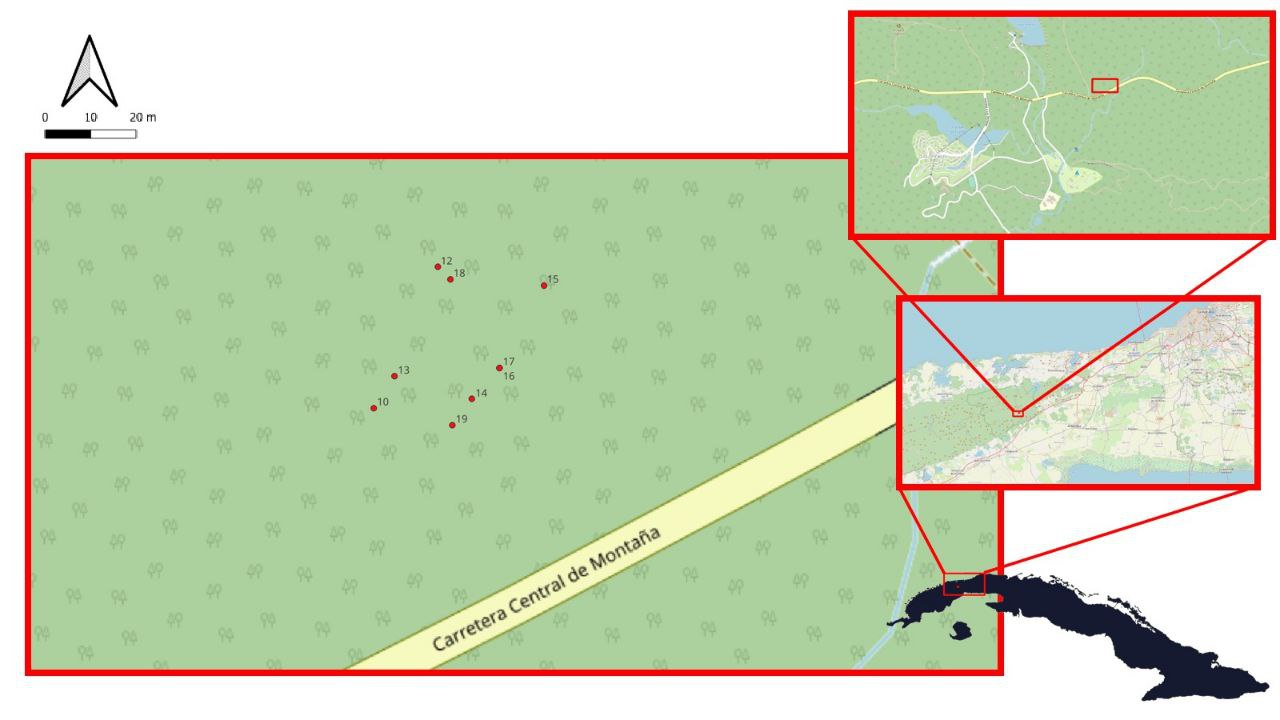
\includegraphics[width=\columnwidth]{Graphics/mic_map.jpg}
    \caption{Distribución Geográfica de los Micrófonos.}
    \label{fig:map}
\end{figure}

Debido a que los micrófonos son omnidireccionales y están situados 
relativamente cercanos entre sí, en cada uno se registran no solamente
los cantos del individuo de Colín más cercano, sino también cantos de especímenes
cercanos, sonidos del ambiente natural de la zona, e incluso ruidos de 
agentes artificales como autos pasando por una carretera cercana.



\section{Motivaciones de la investigación}

Como parte de los estudios sobre la ecología de esta especie de anuros
se quiere profundizar en lo que se conoce sobre las características de sus cantos,
de sus métodos de comunicación y su comportamiento social. Además se quiere 
saber si realmente se organizan en coros, y si ese fuera el caso, analizar la
estructura de dichos coros, la posible existencia de un líder o protagonista,
o de manera general estudiar las interacciones en el sistema formado por los Colines
machos mientras cantan para atraer a las hembras.\\

Hasta el momento, el trabajo para procesar los audios recopilados se realizaba de forma manual
con \emph{softwares} no automáticos. La identificación manual de cada llamado (etiquetado por 
individuo, hora y localización) resulta extremadamente lenta, 
sujeta a errores humanos y poco reproducible. Dichas razones,
sumadas a la búsqueda de avances más eficientes y rigurosos, motivaron el tratamiento
del problema desde un enfoque computacional, para automatizar los procesos
y poder modelar matemáticamente el sistema de interacción entre los Colines.\\ 


\section{Problema científico}

El problema planteado se reduce a, dado un \emph{dataset} de grabaciones
de campo de un coro de Colines hechas con 9 micrófonos omnidireccionales,
procesar los datos para obtener la información de los cantos de cada uno de 
los individuos implicados (momento del canto, frecuencia, energía) para
analizar la estructura de dicho coro. \\

Que los dispositivos de sean omnidireccionales plantea la dificultad de
que en una misma grabación se registra la información de sonidos que no interesan,
como otros animales, autos e incluso Colines que no son los más cercanos al aparato.
Por lo tranto surge la necesidad de diseñar un proceso para discriminar correctamente
estos datos, y obtener una asigación Micrófono-Colín. Además es evidente que se impone
encontrar una forma de eliminar el ruido y “limpiar” los audios. 
También se debe verificar la correcta sincronización de las grabaciones,
pues a pesar de la activación remota y simultánea, el posible error de \emph{hardware}
podría comprometer la precisión de los resultados.\\

Convendría modelar matemáticamente el sistema
para cuantificar las interacciones entre los especímenes y llevar a cabo un estudio
de causalidad. Para ello se propone la utilización de un recurso clásico
de la Física Estadística, el Modelo de Ising. \cite{chau2017inverse}

\section{Objetivos de la tesis}

El objetivo principal de esta tesis es diseñar, implementar y validar un flujo computacional automatizado para la detección, clasificación y análisis de los cantos de apareamiento de \emph{Eleutherodactylus eileenae}, con el fin de reconstruir la estructura de sus coros y modelar las interacciones acústicas entre individuos mediante el enfoque del modelo de Ising.
Para ello se plantean los siguientes objetivos específicos:

\begin{enumerate}
  \item Construir un \emph{dataset} limpio de grabaciones que permita extraer estadísticas fiables y facilitar la interpretación de resultados.
  \item Desarrollar un método de sincronización automática de las señales grabadas por los nueve micrófonos para asegurar la consistencia temporal del \emph{dataset}.
  \item Implementar técnicas de eliminación de ruido de fondo y filtrado de eventos no deseados (otros animales, vehículos, artefactos ambientales).
  \item Diseñar y comparar algoritmos para la obtención de las secuencias de cantos de cada Colín.
  \item Validar la consistencia, precisión y reproducibilidad de los métodos propuestos.
  \item Modelar matemáticamente la red de interacciones acústicas entre individuos utilizando el modelo de Ising:
    \begin{itemize}
      \item Formulación del problema como Principio de Máxima Verosimilitud.
      \item Implementación de algoritmos de Descenso por Gradiente para la inferencia de los parámetros \(J_{ij}\) (interacción entre el individuo $i$ y $j$).
    \end{itemize}
  \item Analizar la idoneidad del modelo de Ising para describir la causalidad en los coros, comparando las interacciones inferidas con comportamientos observados.
  \item Interpretar los resultados y extraer conclusiones ecológicas y computacionales que permitan proponer recomendaciones para estudios bioacústicos futuros.
\end{enumerate}

Para abordar estos objetivos, la tesis se organiza en los siguientes capítulos:
\begin{description}
  \item[Capítulo 1:] \emph{Detección de individuos a partir de señales de audio}. Revisión del estado del arte en detección y clasificación de llamadas bioacústicas.
  \item[Capítulo 2:] \emph{Métodos y metodologías}. Representación de audio como \emph{mel}-espectrogramas, sincronización, eliminación de ruido, diseño de algoritmos de identificación y discriminación de Colines, y formulación del modelo de Ising con su inferencia mediante máxima verosimilitud y descenso por gradiente.
  \item[Capítulo 3:] \emph{Resultados e interpretación}. Evaluación de la sincronización automática, obtención de secuencias de cantos, hipótesis de comportamiento espectral, comparación de algoritmos, pruebas de consistencia y precisión, y análisis de las interacciones inferidas \(\{J_{ij}\}\) en el modelo de Ising.
  \item[Conclusiones y Recomendaciones:] Síntesis de hallazgos, discusión de implicaciones ecológicas y computacionales, limitaciones del estudio y propuestas de trabajo futuro.
\end{description}

% -----------------------------------------------------------------------

